\section{Data Analysis with De-Noising}

In this section we compare results from analysis of raw background merged data sample with files that were de-noised prior to running through CLAS12 reconstruction software. The comparison was done for files with different background merged (namely $45~nA$, $95~nA$ and $150~nA$). The data for raw sample and de-nosied sample was processed with same settings of CLAS12 reconstruction software.

\subsection{Luminosity dependence}

The track reconstruction efficiency was calculated according to Eq.~\ref{eq::eff} for positive and negative charged particles. The results are shown on Figure~\ref{lscan::conv_dn}. 

\begin{figure}[!h]
\begin{center}
 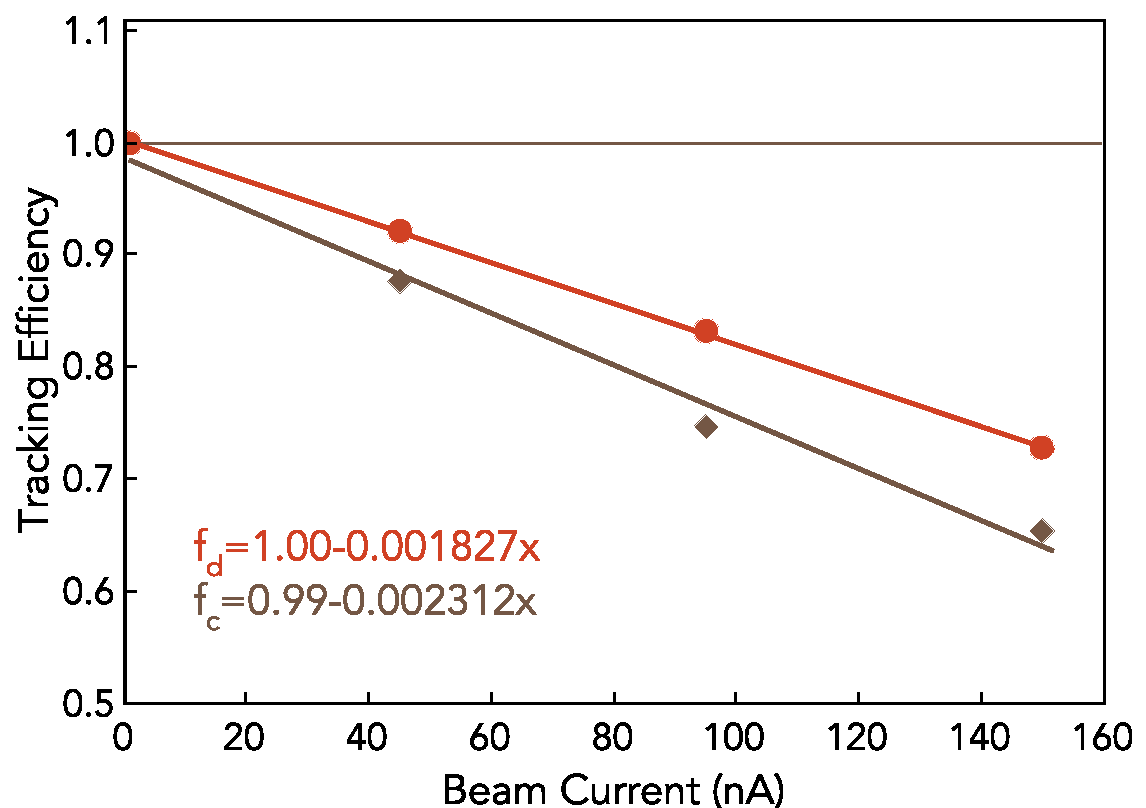
\includegraphics[width=3.1in]{images/figure_lscan_pos.pdf}
 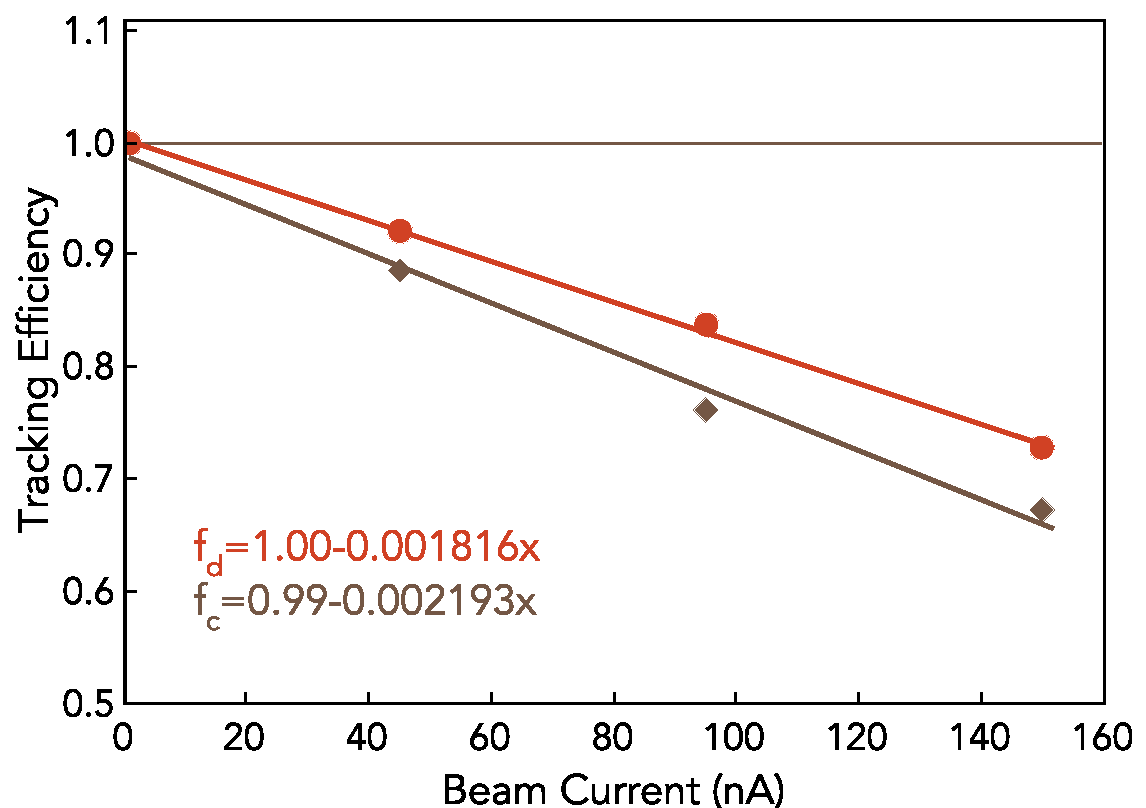
\includegraphics[width=3in]{images/figure_lscan_neg.pdf}
\caption {Tracking efficiency as a function of luminosity (beam current) for positive (a) and negative particle (b).  The efficiency is shown for
conventional algorithm running on background merged files (diamonds), and on files with merged background then de-noised with AI (circles).}
 \label{lscan::conv_dn}
 \end{center}
\end{figure}

As can be seen from the figure the number of reconstructed hadron-electron pairs relative to reconstructed electrons is higher for de-noised data sample compared to the raw data sample. This is due to increased number of clusters reconstructed by conventional clustering algorithm in de-noised data samples. Detailed studies of cluster reconstruction efficiency were performed in our studies of neural network paper. The result show that the slope of efficiency degradation as a function of luminosity is significantly improved in de-noised data sample. It is worth noting that at $90~nA$ the de-noised data sample track reconstruction efficiency is same as for the $45~nA$ when reconstructing raw data sample (without de-noising). This implies that experiment can run at effectively at $90~nA$, collecting data twice faster, while maintaining the same track reconstruction efficiency.

\subsection{Physics Impact}

The processed data was also evaluated to extract physics observables from both data sample to discern the impact on physics for de-noising algorithm. As mentioned before the data selected from Pythia simulation was for the final state $H(e,e^\prime\pi^+\pi^-pX)$. From this sample the missing mass distribution of $H(e,e^\prime\pi^+\pi^-X)$ is analyzed which should show proton mass where the selected reaction was inclusive $\rho$ meson production and some background (above proton mass) where other reactions (with missing neutral particles)  are selected.

\begin{figure}[!h]
\begin{center}
  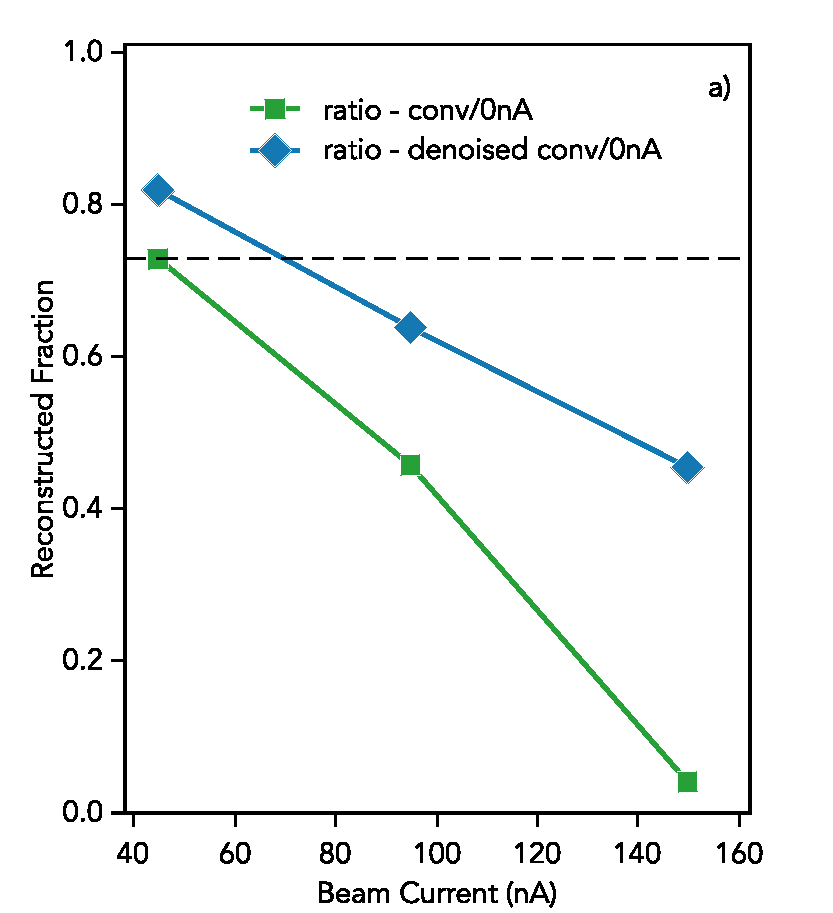
\includegraphics[height=2.8in]{images/graph_mxepipi_dn.pdf}
 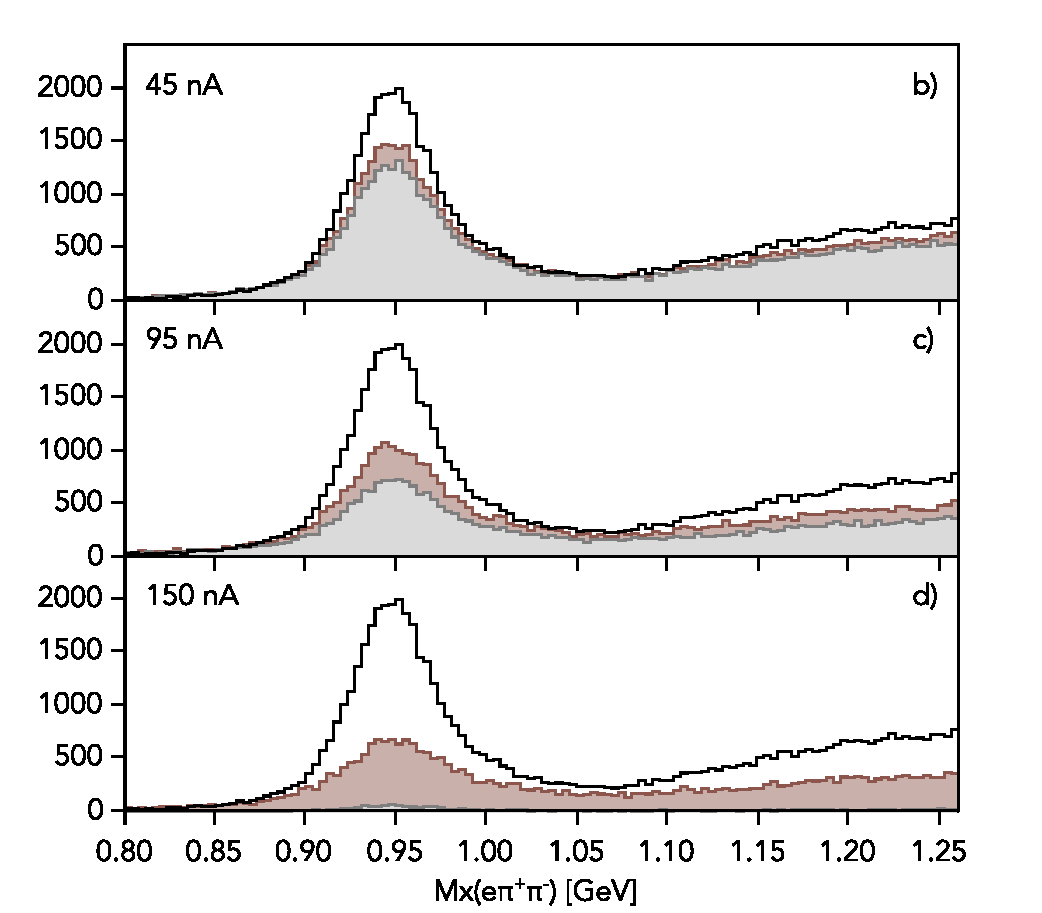
\includegraphics[height=2.8in]{images/plots_mxepipi_dn.pdf}
\caption {Number of reconstructed protons from missing mass of $H(e \rightarrow e^\prime \pi^+\pi^-)$ for background merged files for  $5~nA$, $45~nA$, $95~nA$ and $150~nA$ respectively. The number of protons reconstructed by conventional algorithm after background merging is shown on the top row, and reconstruction after  de-noising drift 
chamber data on the bottom row.}
 \label{physics::conv_dn}
 \end{center}
\end{figure}

On Figure~\ref{physics::conv_dn} the results of analysis are shown, where the missing mass distribution $H(e,e^\prime\pi^+\pi^-)X$ is plotted for both background merged data (top row) and for background merged de-noised data (bottom row) as a function of incident beam current (luminosity).  The scale on all plots is set to the same heigh to visually observe decrease of number of protons reconstructed. 

%\begin{figure}[!ht]
%\begin{center}
 %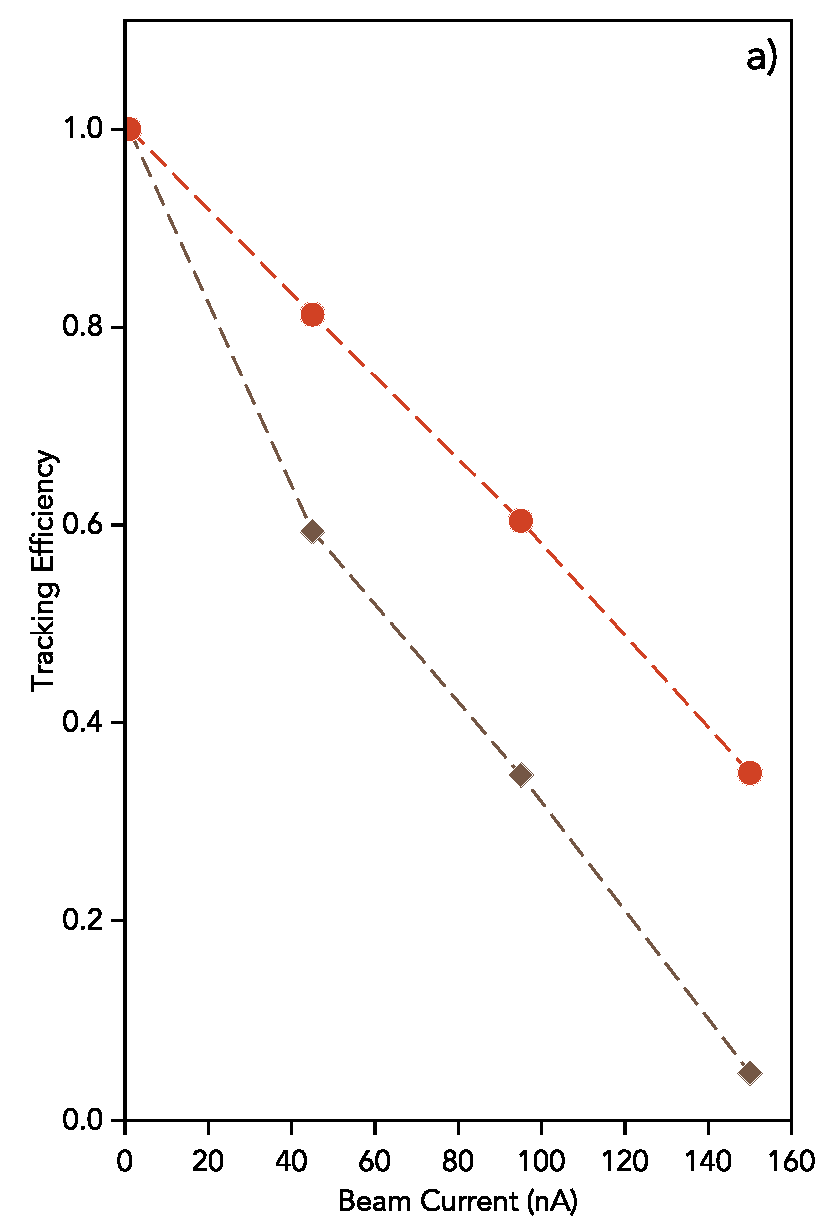
\includegraphics[width=3.1in]{images/figure_phys_scan.pdf}
 %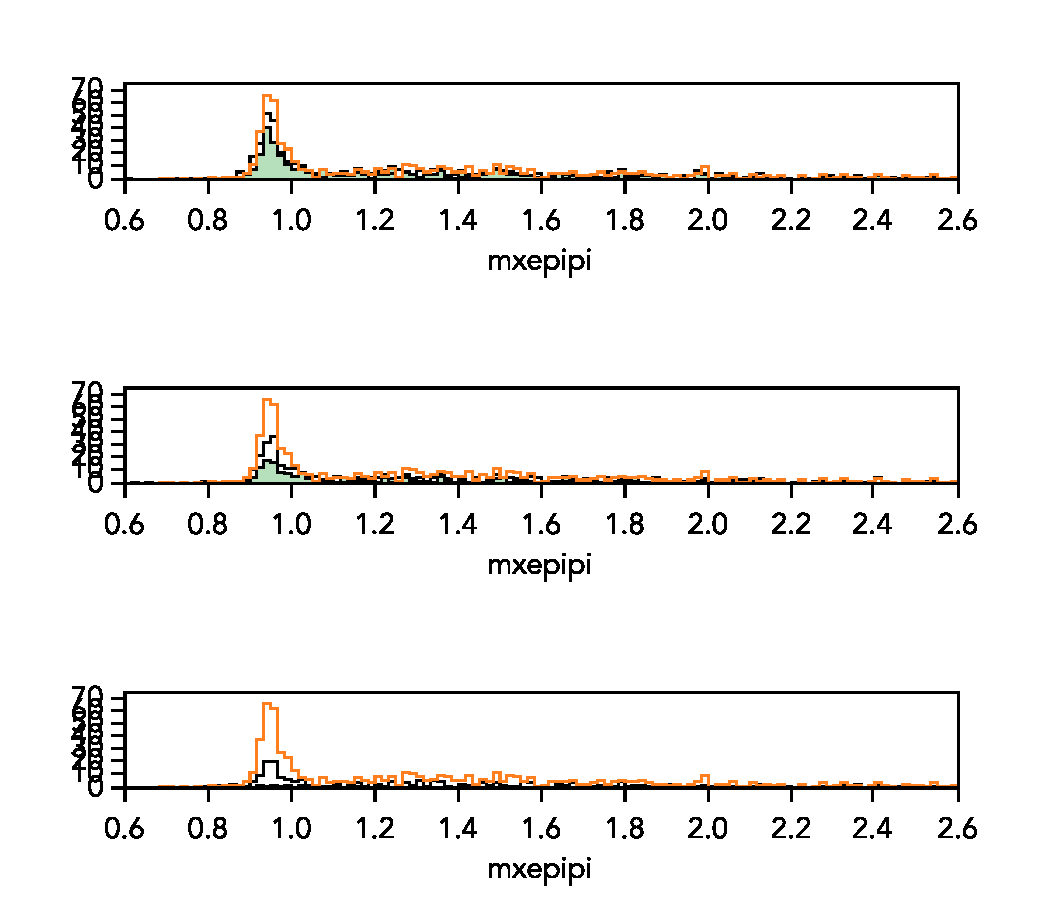
\includegraphics[width=2.5in]{images/figure_phys_conv_compare.pdf}
%\caption {Number of reconstructed protons from missing mass 
%of $H(e e^\prime \pi^+\pi^-)$ for background merged files for 
%$5~nA$, $45~nA$, $95~nA$ and $150~nA$ respectively.}
 %\label{physics::count_raw_dn}
 %\end{center}
%\end{figure}

On Figure~\ref{physics::conv_dn} (a) the dependence is plotted for both data samples, where the points represent number of events under the proton peak normalized to the number of protons reconstructed by the tracking algorithm before background merging procedure (shown on Figure~\ref{physics::count_raw_dn} in the first column).
It is evident from the figure that number of reconstructed protons in the de-noised data at $45~nA$ is $37\%$ larger, and the number of reconstructed protons at $95~nA$ in de-noised data sample is $2\%$ larger than in $45~nA$ background merged files. This result has significant implications on future experiments, since the data can be collected much fasted to reach the required statistical significance for given physics program while saving significant amount of money in accelerator operation costs.




